% Capitulo III: Marco metodologico (maximo 8 paginas)

\chapter{MARCO METODOLÓGICO}

\section{Marco referencial de metodologías aplicadas}

La ruta del proyecto tiene cinco pasos (Figura~\ref{fig:ruta}): definir los requerimientos, evaluar alternativas y elegir una, diseñar la arquitectura, diseñar el modelo y el flujo de datos, y verificar la solución frente a los requerimientos. La guía general es la directriz VDI 2206, porque ordena el paso de los requerimientos a la verificación en sistemas ciberfísicos \cite{vdi2206,graessler2020}. Además, se aplican dos marcos a partes concretas del diseño: la IEC 62264 (ISA-95), para ubicar por niveles el compresor, su controlador, el gateway y la sombra digital \cite{iec62264}; y la ISO 13374, que organiza el procesamiento de datos en adquisición, manipulación, detección de estado, evaluación de salud y recomendación \cite{iso13374}, etapas que corresponden a los módulos de la sombra digital. No se emplean otras metodologías, porque no aportan decisiones al diseño de este proyecto.

\begin{figure}[htbp]
\centering
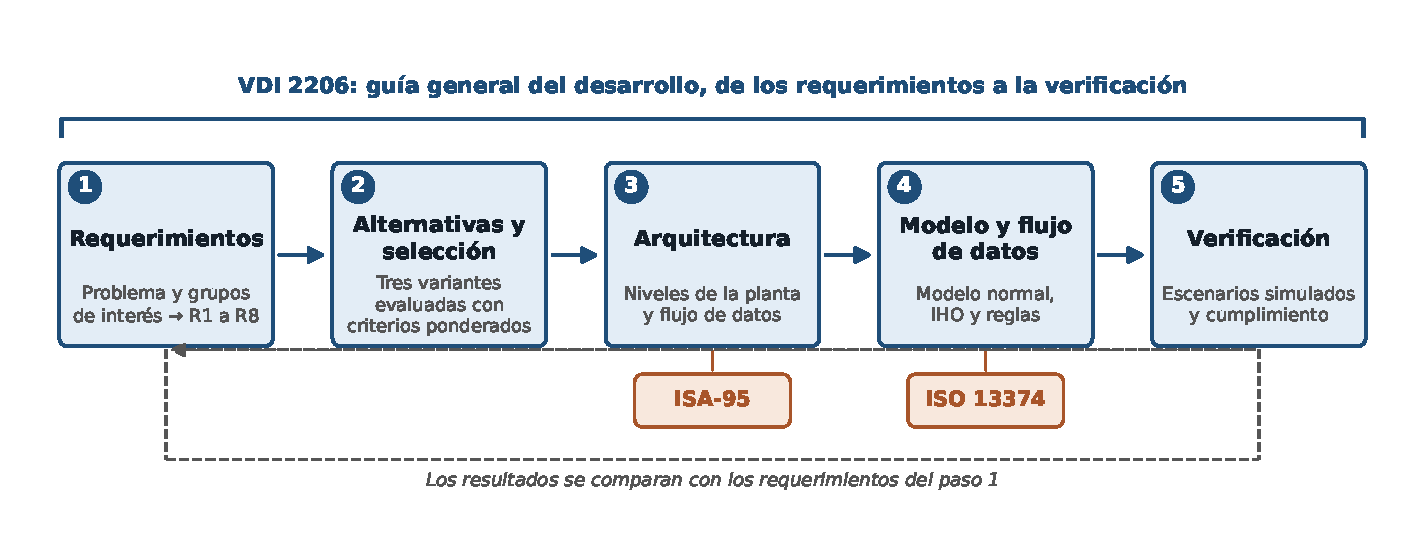
\includegraphics[width=\textwidth]{fig_ruta_metodologica.pdf}
\caption{Ruta metodológica del proyecto}
\label{fig:ruta}
\end{figure}

\section{Requerimientos de la solución}

Los requerimientos se derivaron del problema y de los grupos de interés del Capítulo I (Tabla~\ref{tab:req}).

\begin{table}[htbp]
\centering
\caption{Requerimientos de la sombra digital}
\label{tab:req}
\footnotesize
\renewcommand{\arraystretch}{1.3}
\begin{tabular}{|p{0.7cm}|p{2.2cm}|p{6.0cm}|p{4.2cm}|}
\hline
\textbf{ID} & \textbf{Grupo} & \textbf{Requerimiento} & \textbf{Criterio de verificación} \\ \hline
R1 & Mantenimiento & Detectar desviaciones térmicas antes del aviso del controlador & Anticipación mínima de 7 días \\ \hline
R2 & Mantenimiento & Detectar un aumento sostenido de los ciclos de carga y descarga & Alerta ante un aumento de 20\,\% \\ \hline
R3 & Producción & Evitar alertas sin causa & Menos del 5\,\% del tiempo fuera de verde sin falla \\ \hline
R4 & Operación & No interferir con el control ni las protecciones & Acceso de solo lectura \\ \hline
R5 & Mantenimiento & Presentar la información de forma comprensible & Índice de 0 a 100, causa y acción \\ \hline
R6 & Servicio técnico & Usar las variables que ya registra el controlador & Sin sensores adicionales \\ \hline
R7 & Servicio técnico & Ajustarse a cada equipo con su propio histórico & Calibración con 14 días de datos \\ \hline
R8 & Mantenimiento & Contar con un modelo de referencia confiable & RMSE de validación menor a 2\,K \\ \hline
\end{tabular}
\end{table}

\section{Evaluación y selección de la solución}

Se plantearon tres alternativas. La V1 es un monitoreo básico, con exportación de archivos y umbrales fijos. La V2 es una sombra digital con un gateway de borde, un modelo de comportamiento normal calibrado con el histórico del equipo y reglas expertas. La V3 es un gemelo digital avanzado, con modelo físico detallado, aprendizaje automático y acción automática sobre el controlador. Se evaluaron con criterios ponderados derivados de los requerimientos (Tabla~\ref{tab:eval}), con puntajes de 1 a 5; el valor técnico es el puntaje ponderado dividido entre el máximo posible.

\begin{table}[htbp]
\centering
\caption{Evaluación ponderada de las alternativas}
\label{tab:eval}
\footnotesize
\renewcommand{\arraystretch}{1.3}
\begin{tabular}{|p{5.6cm}|c|c|c|c|}
\hline
\textbf{Criterio} & \textbf{Peso} & \textbf{V1} & \textbf{V2} & \textbf{V3} \\ \hline
Capacidad de anticipación (R1, R2) & 0,30 & 2 & 5 & 5 \\ \hline
Seguridad operativa (R4) & 0,20 & 5 & 5 & 2 \\ \hline
Factibilidad con datos disponibles (R6, R7) & 0,20 & 5 & 4 & 2 \\ \hline
Facilidad de interpretación (R5) & 0,15 & 4 & 4 & 3 \\ \hline
Simplicidad de implementación & 0,15 & 4 & 3 & 1 \\ \hline
\textbf{Valor técnico} & & \textbf{0,76} & \textbf{0,87} & \textbf{0,58} \\ \hline
\end{tabular}
\end{table}

Los pesos y puntajes son valoraciones de diseño del equipo, no mediciones. La V2 obtuvo el mayor valor técnico: frente a V1, detecta que la temperatura se aleja de lo esperado aunque siga dentro del rango permitido, y frente a V3, no actúa sobre el controlador y no necesita datos de fallas que no están disponibles. Según Kritzinger et al.~\cite{kritzinger2018}, la V2 es una sombra digital, ya que los datos fluyen del compresor al modelo y la decisión queda en manos del personal.

\section{Arquitectura}

La Figura~\ref{fig:isa95} ubica los componentes en los niveles de la IEC 62264. El compresor y sus sensores forman el nivel 0; su controlador con softPLC, que conserva la regulación y las protecciones, el nivel 1. En el nivel 2, un gateway de borde lee el controlador por Ethernet mediante Modbus TCP u OPC UA \cite{iec62541}; en el nivel 3 está la sombra digital; y el nivel 4 recibe las recomendaciones para la gestión del mantenimiento. La sincronización es unidireccional y se hace cada 10 minutos, porque la degradación evoluciona en días y no requiere tiempo real.

\begin{figure}[htbp]
\centering
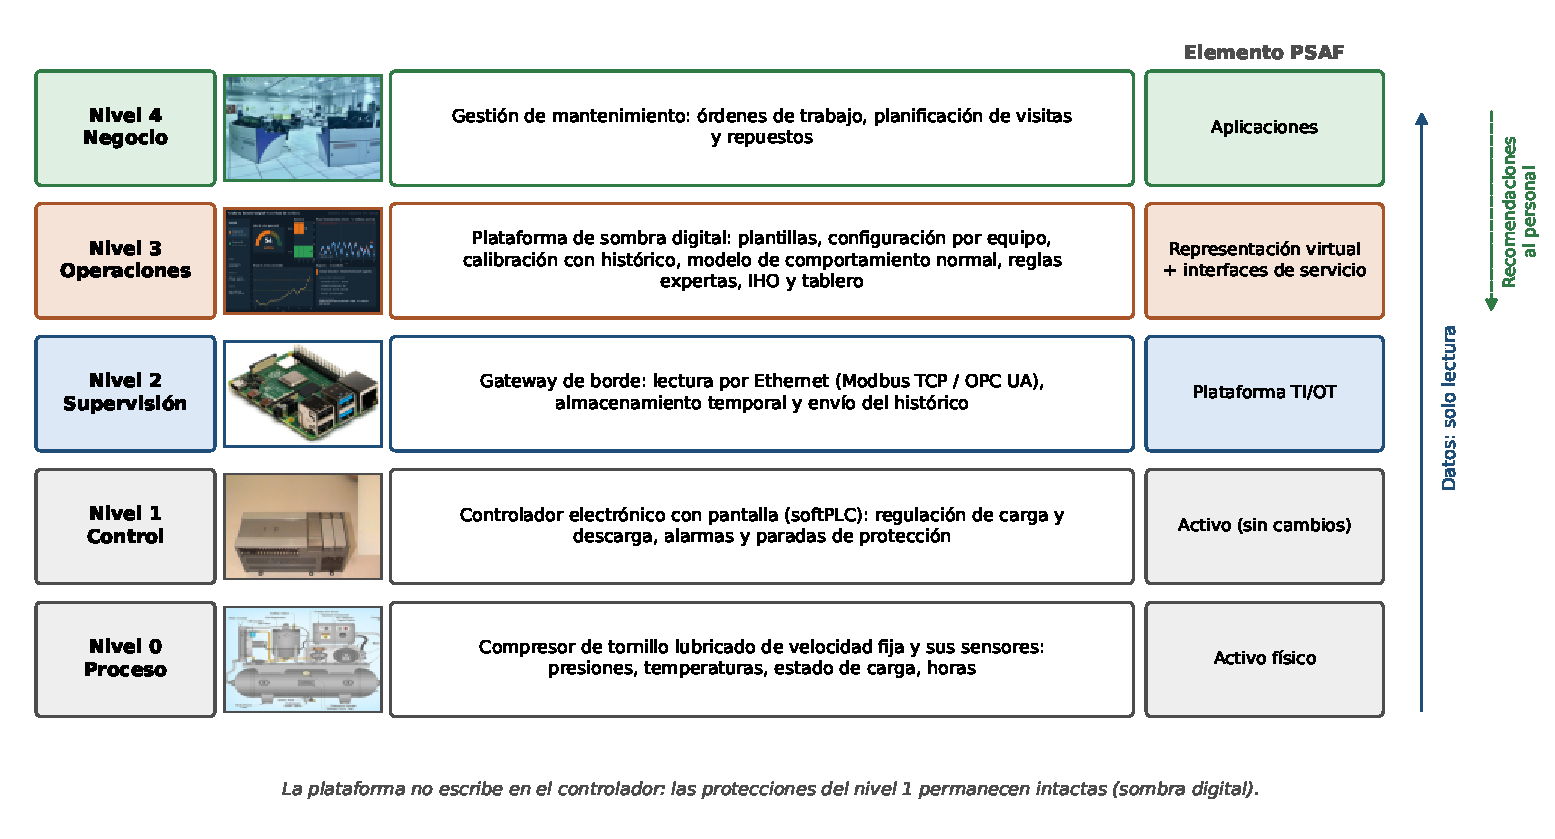
\includegraphics[width=\textwidth]{fig_arquitectura_isa95_fotos.pdf}
\caption{Arquitectura según los niveles de ISA-95. Imágenes: B. S. Elliott (CC BY-SA 4.0), Wikimedia Commons (CC BY-SA 3.0), Laserlicht (CC BY-SA 4.0) y Z22 (CC BY-SA 4.0), vía Wikimedia Commons; tablero: elaboración propia}
\label{fig:isa95}
\end{figure}

\section{Diseño del modelo y del flujo de datos}

El flujo sigue las cinco etapas de la ISO 13374. En la \emph{adquisición}, el gateway lee la temperatura de salida del elemento, la temperatura ambiente, la presión de descarga, el estado de carga o descarga y los avisos del controlador. En la \emph{manipulación}, los datos se agregan en ventanas de 10 minutos. En la \emph{detección de estado}, un modelo de comportamiento normal estima la temperatura que debería tener el compresor según las condiciones de operación. Como la temperatura depende de la temperatura ambiente, del tiempo en carga y de la presión, se plantea una regresión lineal, calibrada con 14 días de histórico del equipo:
\begin{equation}
\hat{T}_e = \beta_0 + \beta_1\,T_{amb} + \beta_2\,FC + \beta_3\,p
\label{eq:modelo}
\end{equation}
donde $\hat{T}_e$ es la temperatura esperada en °C, $T_{amb}$ la temperatura ambiente, $FC$ la fracción de tiempo en carga en la ventana y $p$ la presión media en bar(g). Se eligió una regresión por ser fácil de explicar y por no requerir datos de fallas.

La diferencia entre la temperatura medida y la esperada, $r_k = T_{e,k} - \hat{T}_{e,k}$, se suaviza con un promedio móvil exponencial, $D_k = \lambda\, r_k + (1-\lambda)\, D_{k-1}$ con $\lambda = 0{,}02$, para obtener la desviación térmica sostenida. Para el ciclaje se usa el aumento relativo de ciclos de carga por hora respecto al periodo de calibración, $\Delta c = \bar{c}/c_{ref} - 1$. En la \emph{evaluación de salud}, ambos se convierten en subíndices de 0 a 100 y el índice de salud operacional (IHO) lo define el peor de los dos:
\begin{equation}
H_T = 100\left[1 - \min\!\left(\max\!\left(\frac{D_k}{12\,\mathrm{K}}, 0\right), 1\right)\right], \quad
H_C = 100\left[1 - \min\left(\max\left(\Delta c, 0\right), 1\right)\right]
\end{equation}
\begin{equation}
\mathrm{IHO} = \min(H_T, H_C)
\end{equation}

En la \emph{recomendación}, un nivel se confirma si se mantiene 6 horas continuas y se asocia con una acción (Tabla~\ref{tab:semaforo}). Una base de reglas expertas añade las causas probables: una temperatura mayor a la esperada apunta al enfriador, la ventilación, el aceite o la válvula termostática; un aumento de ciclos, a la pérdida de capacidad efectiva del sistema, a una banda de presión estrecha o a un cambio en la demanda. Las alarmas y paradas siguen a cargo del controlador.

\begin{table}[htbp]
\centering
\caption{Niveles del índice de salud operacional}
\label{tab:semaforo}
\footnotesize
\renewcommand{\arraystretch}{1.3}
\begin{tabular}{|p{1.4cm}|p{1.6cm}|p{2.1cm}|p{2.0cm}|p{5.4cm}|}
\hline
\textbf{Nivel} & \textbf{IHO} & \textbf{Desviación térmica} & \textbf{Aumento de ciclos} & \textbf{Acción recomendada} \\ \hline
Verde & 80 o más & menos de 2,4\,K & menos de 20\,\% & Operación normal \\ \hline
Amarillo & 60--80 & 2,4--4,8\,K & 20--40\,\% & Revisar en la próxima ronda \\ \hline
Naranja & 40--60 & 4,8--7,2\,K & 40--60\,\% & Programar una inspección \\ \hline
Rojo & menos de 40 & más de 7,2\,K & más de 60\,\% & Revisión prioritaria antes de una parada \\ \hline
\end{tabular}
\end{table}

\section{Origen de los datos y de los parámetros}

No se dispone de datos de un equipo en operación, por lo que la verificación usa datos sintéticos generados en MATLAB con el modelo de la Sección~\ref{sec:sim}. Se generan las mismas variables que registra un controlador de compresor: presión, temperatura de salida del elemento, temperatura ambiente y estado de carga o descarga. Existen conjuntos públicos de datos reales con variables de este tipo, como MetroPT-3, que registra presión, temperatura del aceite, corriente del motor y señales de carga y descarga de la unidad de aire de un tren \cite{metropt3}; estos datos o los registros de una auditoría energética permitirían calibrar la sombra digital en una etapa posterior. La Tabla~\ref{tab:origen} indica el origen de cada parámetro; los que no tienen fuente son supuestos de diseño, que en una aplicación real se reemplazan por la ficha técnica y la configuración del controlador del equipo.

\begin{table}[htbp]
\centering
\caption{Origen de los parámetros de la simulación}
\label{tab:origen}
\footnotesize
\renewcommand{\arraystretch}{1.3}
\begin{tabular}{|p{3.5cm}|p{2.8cm}|p{6.6cm}|}
\hline
\textbf{Parámetro} & \textbf{Valor} & \textbf{Origen} \\ \hline
Regulación del compresor & Carga y descarga entre dos presiones & Modelo de la operación en carga y descarga \cite{liang2019} \\ \hline
Banda de presión & 6,5 a 7,5\,bar(g) & Supuesto de diseño, dentro de las presiones de trabajo industriales; en MetroPT-3 se documentan umbrales de 7 y 8,2\,bar \cite{metropt3} \\ \hline
Ciclos de carga por hora & Cerca de 8 por hora & Resultado de la simulación; del orden de los 6 a 8 arranques por hora que se recomienda como criterio de diseño del almacenamiento \cite{marshall2013} \\ \hline
Escenario de ciclaje & Pérdida de volumen útil & La pérdida de capacidad efectiva, como la que causa la caída de presión en filtros, aumenta los ciclos por hora \cite{marshall2013} \\ \hline
Temperatura de salida & Ambiente más un incremento en carga y otro en descarga & Calentamiento por compresión; la temperatura del aceite influye en el desempeño \cite{kumar2022}. Los incrementos son supuestos de diseño \\ \hline
Caudal, volumen de la red, constantes de tiempo, demanda y ruido & Valores típicos & Supuestos de diseño del orden de un compresor de 45\,kW \\ \hline
Aviso por alta temperatura & 110\,°C & Supuesto; se reemplaza por el valor configurado en el controlador \\ \hline
\end{tabular}
\end{table}

\section{Modelo de simulación y plan de verificación}
\label{sec:sim}

La presión de la red se modela con la regulación por carga y descarga, y la temperatura del elemento como un sistema de primer orden:
\begin{equation}
\frac{dp}{dt} = \frac{p_{atm}\,(Q_c - Q_d)}{60\,V}, \qquad
\frac{dT_e}{dt} = \frac{T_{ss} - T_e}{\tau}
\end{equation}
donde $Q_c$ es el caudal del compresor, $Q_d$ la demanda, $V$ el volumen útil de la red, $T_{ss}$ la temperatura de equilibrio y $\tau$ la constante de tiempo. Desde el día 30 se simulan dos degradaciones graduales: un incremento térmico de hasta 30\,K, por pérdida de capacidad del enfriador, y una reducción del volumen útil hasta el 40\,\%.

La verificación evalúa el modelo con datos no usados en su calibración ($R^2$ y RMSE); registra el día en que se confirma cada nivel frente al inicio de la falla y al aviso del controlador; repite el análisis en 10 simulaciones por escenario, más una prueba de robustez con efectos térmicos no incluidos en el modelo; y contrasta los resultados con la Tabla~\ref{tab:req}. La validación con datos reales queda como etapa posterior a este proyecto.
